\section{Лабораторная работа №5}
Экспериментальное исследование статически неопределимой балки

Цель работы: теоретическое и экспериментальное определение реактивного момента в заделке и прогиба балки в нескольких точках.

Оборудование и инструменты: специальный стенд, индикаторы перемещений часового типа, штангенциркуль, измерительная линейка.

\subsection{Теоретические сведения}
Отбросив правую опору и заменив её силой $ X_1 $, получим эквивалентную статически определимую систему (рис. \ref{fig:shear-scheme-equal}).
Величину силы $ X_1 $ находят из канонического уравнения \[ \Delta_{1P} + \delta_{11} X_1 = 0, \]
Умножая эпюру $ P $ на эпюру $ 1 $ получим
\begin{equation}
    \Delta_{1P} = \frac{1}{EI_X} \left(\frac{1}{2} \frac{l}{2} \frac{Pl}{2}\right) \frac{5}{6} l = \frac{5}{48} \frac{Pl^3}{EI_X}
\end{equation}
Аналогично умножим эпюру 1 на себя
\begin{equation}
    \delta_{11} = \frac{1}{EI_X} \left(\frac{1}{2}ll\right) \frac{2}{3}l = \frac{l^3}{3EI_X}
\end{equation}
\begin{equation}
    X_1 = \frac{5}{16}P.
\end{equation}
По эпюре видно, что максимальный момент возникает в заделке и составляет $ M_{max} = -\frac{3}{16}Pl $.
\begin{align*}
    V_A = \frac{25}{6144}\frac{Pl^3}{EI_X} \\
    V_B = \frac{56}{6144}\frac{Pl^3}{EI_X} \\
    V_C = \frac{43}{6144}\frac{Pl^3}{EI_X} \\
\end{align*}

\begin{figure}[!ht]
    \centering
    \begin{subfigure}[b]{0.4\textwidth}
        \centering
        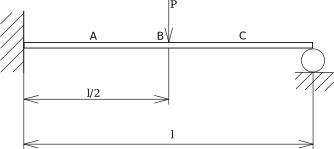
\includegraphics[width=\textwidth]{shear-scheme.pdf}
        \caption{}
        \label{fig:shear-scheme}
    \end{subfigure}
    \hspace{0.1\textwidth}
    \begin{subfigure}[b]{0.4\textwidth}
        \centering
        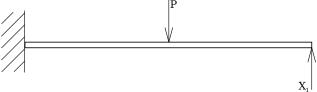
\includegraphics[width=\textwidth]{shear-scheme-equal.pdf}
        \caption{}
        \label{fig:shear-scheme-equal}
    \end{subfigure}
    \hspace{0.1\textwidth}
    \begin{subfigure}[b]{0.4\textwidth}
        \centering
        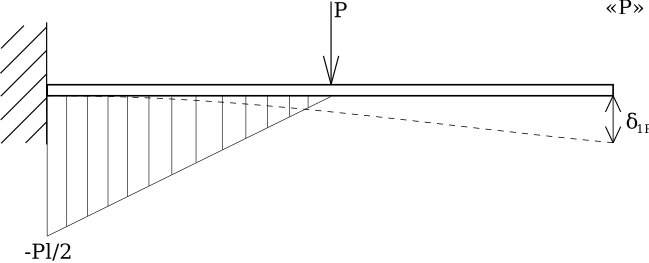
\includegraphics[width=\textwidth]{moment-diagram-of-forces.pdf}
        \caption{}
        \label{fig:moment-diagram-of-forces}
    \end{subfigure}
    \hspace{0.1\textwidth}
    \begin{subfigure}[b]{0.4\textwidth}
        \centering
        \includegraphics[width=\textwidth]{moment-diagram-of-unit-force.pdf}
        \caption{}
        \label{fig:moment-diagram-of-unit-force}
    \end{subfigure}
    \hspace{0.1\textwidth}
    \begin{subfigure}[b]{0.4\textwidth}
        \centering
        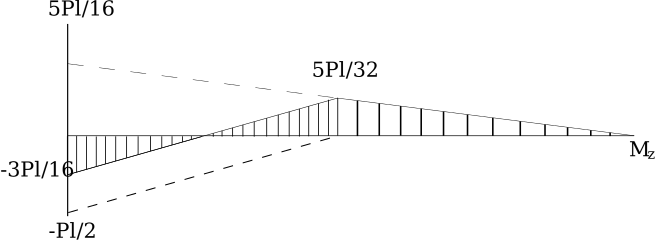
\includegraphics[width=\textwidth]{total-moment-diagram.pdf}
        \caption{}
        \label{fig:total-moment-diagram}
    \end{subfigure}
    \hspace{0.1\textwidth}
    \begin{subfigure}[b]{0.4\textwidth}
        \centering
        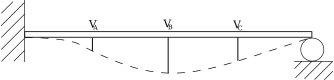
\includegraphics[width=\textwidth]{elastic-line.pdf}
        \caption{}
        \label{fig:elastic-line}
    \end{subfigure}
    \hspace{0.1\textwidth}
    \begin{subfigure}[b]{0.4\textwidth}
        \centering
        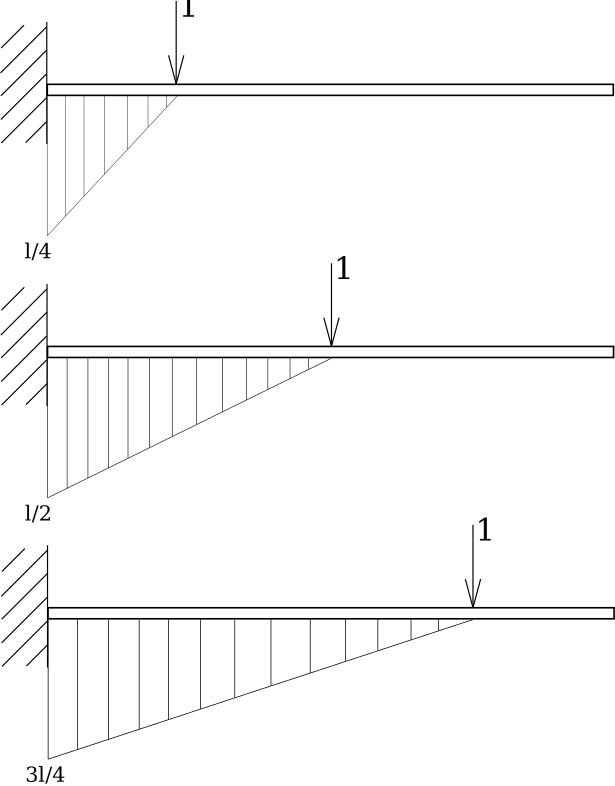
\includegraphics[width=\textwidth]{moment-diagram-of-unit-force-in-points.pdf}
        \caption{}
        \label{fig:moment-diagram-of-unit-force-in-points}
    \end{subfigure}
    \hspace{0.1\textwidth}
    \caption{Раскрытие статической неопределимости и построение упругой линии балки:
    а "--- схема нагружения статически неопределимой балки;
    б "--- эквивалентная схема;
    в "--- эпюра моментов от заданных сил;
    г "--- эпюра моментов от единичной силы;
    д "--- итоговая эпюра моментов;
    е "--- упругая линия балки;
    ж\==и "--- эпюры моментов от единичной силы в точках искомых перемещений.}
    \label{fig:moment-diagrams-and-elastic-line}
\end{figure}

\subsection{Лабораторный стенд}
Экспериментальную проверку полученного теоретического решения проводят на лабораторном стенде.
Экспериментальный стенд реализует расчётную схему при условии, что левая опора представляет собой <<жёсткую заделку>>.
Настенде опора шарнирная.
Для воспроизведения условий <<жёсткой заделки>> на стенде предусмотрена возможность угла поворота левого конца балеи с помощью выносимого рычага 5 и груза 7 (рис. \ref{fig:scheme}).
Угол поворота балки на левой опоре фиксируется индикатором 9.

\begin{figure}[!ht]
    \centering
    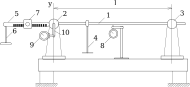
\includegraphics[width=0.8\textwidth]{scheme.pdf}
    \caption{Схема лабораторной установки для проверки принципа взаимности перемещений:
        1 "--- испытуемый стержень;
        2, 3 "--- опоры;
        4 "--- подвеска для грузов;
        5 "--- рычаг;
        6 "--- подвижный груз;
        8, 9 "--- индикаторы.}
        \label{fig:scheme}
    \end{figure}

\subsection{Выполнение работы}

1. Установлю подвеску без груза $P_0$ в середине балки, зафиксирую положение груза $Q$ на рычаге, установлю нулевое положение индикатора угла поворота.
Результаты запишу в табл. \ref{tab:lab5-reactive-moment}.

2. Нагружу балку поперечной силой $P_1 = P_0 + P$.

3. Зафиксирую величину угла поворота левого конца балки.
Занесу данные в табл. \ref{tab:lab5-reactive-moment}.

4. Смещая по рычагу груз $Q$, установлю начальное показание угла поворота.
Зафиксирую новое положение груза.
Вычислю смещение $C$ груза $Q$ и занесу данные в табл. \ref{tab:lab5-reactive-moment}.

5. Вычислю экспериментальную величину реактивного момента $M = QC$ и сравню его с теоретической величиной $M = -\frac{3 P l}{16}$ и найду погрешность
\[
    \delta_M = \frac{|1500 - 1600|}{1500} \cdot 100~\% = 6.6~\%
\]

\begin{table}[!ht]
    \centering
    \caption{Измерение реактивного момента}
    \label{tab:lab5-reactive-moment}
    \begin{tabular}{|m{0.5\textwidth}|c|}
        \hline
        \multicolumn{1}{|c|}{Параметры}                                                & Результаты измерений \\ \hline
        Положение груза $Q$ при начальной нагрузке $P_0$ (вес подвески), мм            & 70 \\ \hline
        Показание индикатора угла поворота при $P_0$, число делений                    & 0 \\ \hline
        Показания индикатора угла поворота при $P_1 = P_0 + P$, число делений          & 133 \\ \hline
        Положение груза $Q$ при компенсации угла поворота, мм                          & 230 \\ \hline
        Смещение $C$ груза $Q$, мм                                                     & 160 \\ \hline
        Реактивный момент в заделке $M = QC$, Н$\cdot$мм                               & 1600 \\ \hline
        Теоретическое значение реактивного момента $M = -\frac{3 P l}{16}$, Н$\cdot$мм & 1500 \\ \hline
    \end{tabular}
\end{table}

\begin{table}[!ht]
    \centering
    \caption{Измерение прогиба балки}
    \label{tab:lab5-flexure}
    \begin{tabular}{|l|l|c|c|c|}
        \hline
        \multicolumn{2}{|c|}{\multirow{2}{*}{Измеряемый параметр}} & \multicolumn{3}{c|}{Точки измерений} \\ \cline{3-5}
        \multicolumn{2}{|c|}{}                                     & A & B & C \\ \hline
        \multicolumn{2}{|m{0.45\textwidth}|}{Показания индикатора прогиба при $P_0$ и начальном положении груза Q}                                       & 0   & 0   & 0 \\ \hline
        \multicolumn{2}{|m{0.45\textwidth}|}{Показание индикатора прогиба при $P_1 = P_0 + P$}                                                           & 416 & 567 & 415 \\ \hline
        \multicolumn{2}{|m{0.45\textwidth}|}{Показания индикатора прогиба при $P_1 = P_0 + P$ и компенсации угла поворота введением реактивного момента} & 302 & 305 & 214 \\ \hline
        \multicolumn{5}{|c|}{$M = QC$} \\ \hline
        \multirow{2}{*}{Прогиб балки в точке} & эксперимент & $1.14$ & $2.62$ & $2.01$ \\ \cline{2-5}
                                              & теория      & $1.16$ & $2.59$ & $1.99$ \\ \hline
    \end{tabular}
\end{table}

Вывод: в результате исследования статически неопределимой балки определили теоретическую и экспериментальную величины реактивного момента с погрешностью, равной $\delta_M = 6.6~\%$.

Наибольшее перемещение, имеет точка B, а наименьшее "--- точка A.
Погрешность, причинами которой служат трение в опорах, тип правой опоры (шарнирно-подвижная), а также человеский фактор, носит случайный характер.
